
\section{Empfohlene Technologien}

Es existiert eine Reihe von quelloffenen und kostenfreien Anwendungen,
welche für die uns bevorstehende Aufgabe verwendet werden können.
Im Folgenden findet eine Auflistung dieser Anwendungen in Unterabschnitten
statt, weil sowohl die Anwendungen selbst als auch die Entscheidung
ihrer Verwendung erklärt werden müssen.

\subsection{Lyx (Textverarbeitungsprogramm)}

Die zu digitalisierenden Werke müssen mit einem Textverarbeitungsprogramm
niedergeschrieben werden. Da die Digitalisierung eines Buches als
Gemeinschaftsaufgabe gelöst werden sollte und folglich mehrere Personen
daran arbeiten, muss der niedergeschriebene Quelltext gut per \emph{Versionskontrolle}
(dazu später mehr) verwaltet werden können. Das geht am einfachsten,
wenn es sich um einfachen Text handelt.

Nun zu den Programmen \TeX , \LaTeX{} und Lyx. \TeX{} ist kurz beschrieben
ein Programm, mit dem sogenannte Makros definieren kann, um einfachen
Text unter Verwendung dieser Makros zu formatieren. \LaTeX{} ist quasi
eine Erweiterung von \TeX{} und eigene Makros bereits definiert, die
wir nutzen werden, um einfachen Text zu formatieren. LyX ist eine
grafische Benutzeroberfläche, die uns hilft, ohne großes Wissen über
die Makros, Text zu formatieren.

Diese Anleitung, welche Sie gerade lesen, wurde ebenfalls mit Lyx
erstellt und nach \LaTeX{} exportiert. Die erzeugte Datei trägt den
Dateipostfix \texttt{tex}. Sie können eine solche Datei mit jedem
normalen Texteditor öffnen und sich den Inhalt anschauen.

Programme wie etwas \emph{Libre Office Writer} und \emph{Microsoft
Office Word} verwenden ein ganz eigenes Dateiformat, welches binär
kodiert ist und welches Sie eben nicht mit jedem Texteditor öffnen
können.

\begin{figure}
\centering{}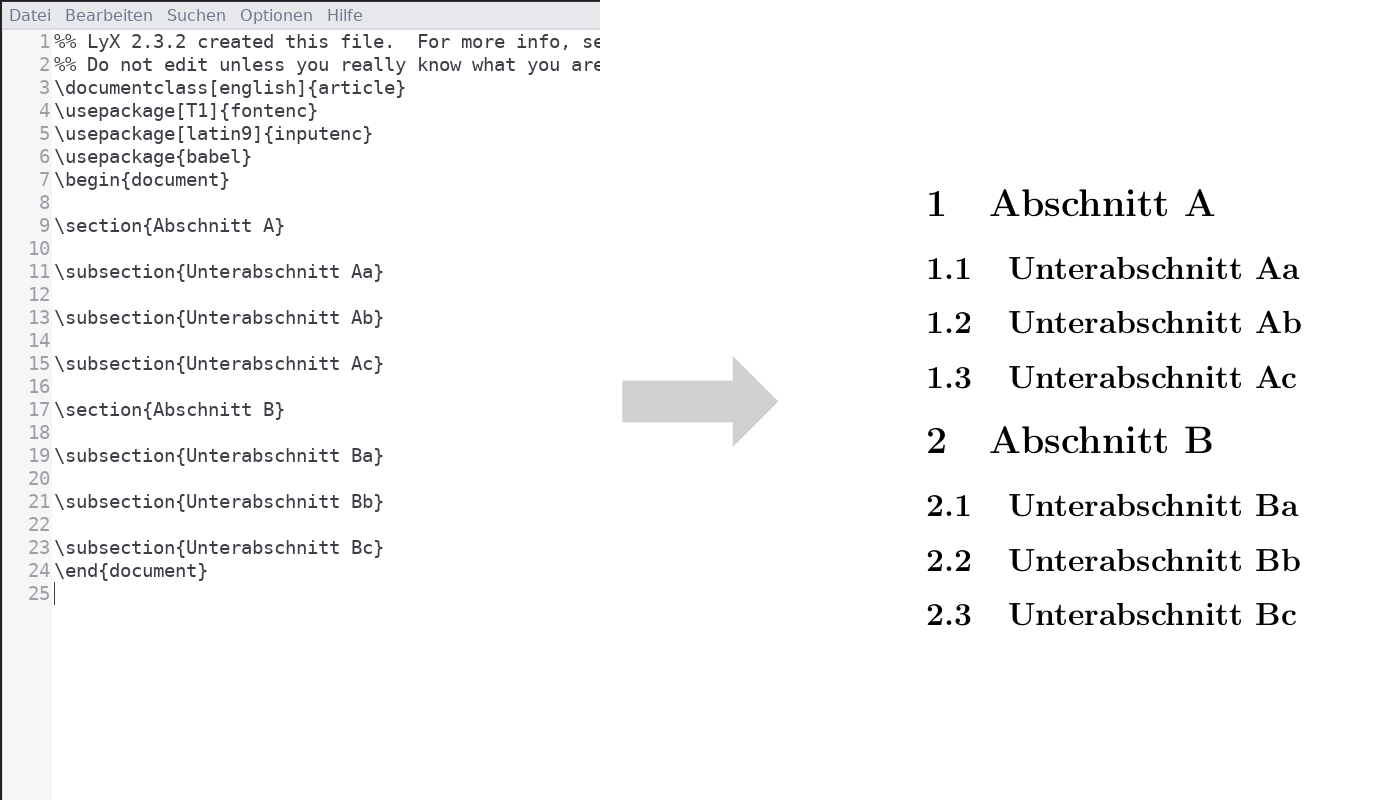
\includegraphics{image_1}\caption{einfacher Text mit Makros nach PDF übersetzt}
\end{figure}


\subsection{Git (Versionskontrolle)}
